\chapter{Integration}

\section{Définition}

\defn{Primitive}{
    Soient $f$ et $F$ deux fonctions définies sur un intervalle $I$ de $\mathbb{R}$ et à valeurs dans $\mathbb{R}$. On dit que $F$ est une primitive de $f$ sur l'intervalle $I$ si $F$ est dérivable sur $I$ et si on a :

$$
\forall x \in I, F^{\prime}(x)=f(x)
$$
}



Toutes les primitives de $f$ sont définies à une constante près, c'est-à-dire que si $F$ est une primitive de $f$, alors, quel que soit $k \in \mathbb{R}$, la fonction $G: x \mapsto F(x)+k$ est également une primitive de $f$.

\defn{Intégrale}{
    Soit $f$ une fonction définie sur un intervalle $I$ de $\mathbb{R}$ et admettant des primitives sur $I$. Soient $(a, b) \in I^2$ et $F$ une primitive de $f$ sur $I$. On appelle intégrale de $a$ à $b$ de $f$, le nombre :

$$
F(b)-F(a)
$$

que l'on notera:

$$
\int_a^b f(x) \mathrm{d} x
$$
}

\begin{figure}[H]
    \centering
    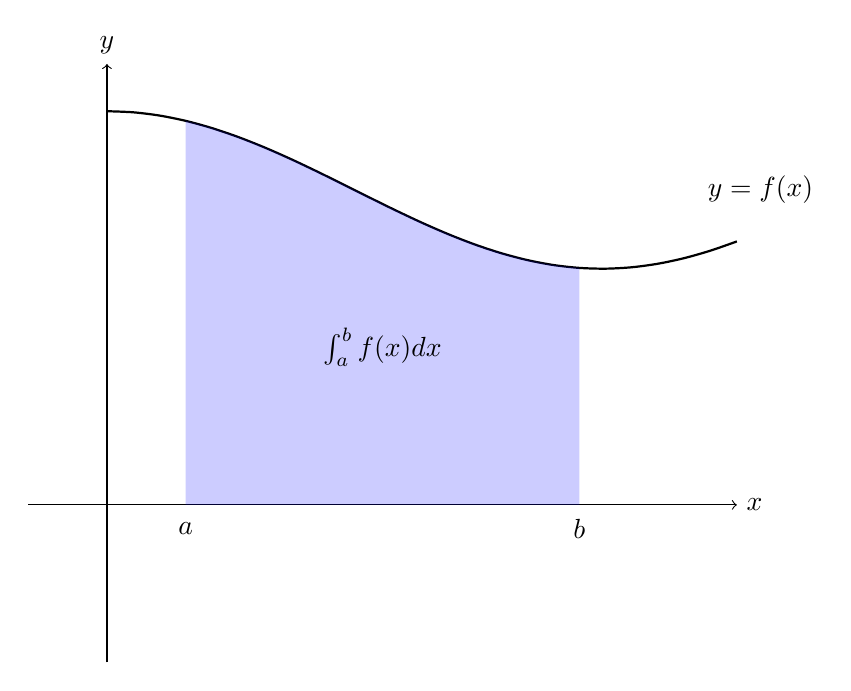
\begin{tikzpicture}[scale=2]
        % Draw the x-axis
        \draw[->] (-0.5,0) -- (4,0) node[right] {$x$};
        
        % Draw the y-axis
        \draw[->] (0,-1) -- (0,2.8) node[above] {$y$};
        
        % Draw the function
        \draw[domain=0:4, smooth, thick] plot (\x, {0.5*cos(\x r) +2});
        
        % Shade the area under the curve
        \fill [blue, opacity=0.2, domain=0.5:3, variable=\x]
        (0.5, 0)
        -- plot ({\x}, {0.5*cos(\x r) +2})
        -- (3, 0)
        -- cycle;

        % Add labels
        \node at (4.15, 2) {$y = f(x)$};
        \node at (0.5, -0.15) {$a$};
        \node at (3, -0.15) {$b$};
        \node at (1.75, 1) {$\int_{a}^{b} f(x) dx$};
      \end{tikzpicture}
\end{figure}

L'intégrale de $f$ entre $a$ et $b$ correspond en fait à l'aire algébrique sous la courbe de $f$.

\thmr{Propriétés de l'intégrale}{int}{
    Soient $f$ et $g$ deux fonctions continues sur un intervalle $I$ de $\mathbb{R}$, et $a, b, c$ appartenant à $I$.
On a :
- Linéarité :

$$
\forall(\lambda, \mu) \in \mathbb{R}^2, \int_a^b(\lambda f(x)+\mu g(x)) \mathrm{d} x=\lambda \int_a^b f(x) \mathrm{d} x+\mu \int_a^b g(x) \mathrm{d} x
$$

- Relation de Chasles:

$$
\int_a^c f(x) \mathrm{d} x=\int_a^b f(x) \mathrm{d} x+\int_b^c f(x) \mathrm{d} x
$$

- Monotonie : si

$$
\forall x \in[a, b], f(x)<g(x)
$$

alors :

$$
\int_a^b f(x) \mathrm{d} x<\int_a^b g(x) \mathrm{d} x
$$


- Inégalité triangulaire:

$$
\left|\int_a^b f(x) \mathrm{d} x\right|<\int_a^b|f(x)| \mathrm{d} x
$$
}

\section{Calcul}

\subsection{Existence}
On ne discutera pas ici tous les critères et théorèmes relatifs à l'existence de l'intégrale d'une fonction sur un intervalle donné, et on s'en tiendra simplement aux points suivants :

\begin{itemize}
    \item Si $f$ est une fonction continue sur un intervalle fermé $[a, b]$, on peut calculer sans risque l'intégrale de $f$ sur $[a, b]$. Idem lorsque la fonction $f$ est continue par morceaux sur $[a, b]$.
    \item Il faut vérifier l'existence de l'intégrale lorsque $f$ est définie sur un intervalle ouvert par exemple $] a, b]$. Tous les cas peuvent se produire ! Exemples :

    $$
    \int_0^1 \frac{1}{x} \mathrm{~d} x
    $$
    
    diverge, car une primitive de $x \mapsto \frac{1}{x}$ est $x \mapsto \ln (x)$ et : $\forall a>0, \ln (1)-\ln (a)=-\ln (a)$, qui tend vers $+\infty$ lorsque $a$ tend vers 0 . L'intégrale diverge... mais :
    
    $$
    \int_0^1 \frac{1}{\sqrt{x}} \mathrm{~d} x
    $$
    
    converge, car une primitive de $x \mapsto \frac{1}{\sqrt{x}}$ est $x \mapsto 2 \sqrt{x}$ et : $\forall a>0,2(\sqrt{1}-\sqrt{a})=2-2 \sqrt{a}$, qui tend vers 2 lorsque $a$ tend vers 0 .
    
    $$
    \int_1^{+\infty} \frac{1}{x^2} \mathrm{~d} x
    $$
    
    converge. En effet, une primitive de $x \mapsto \frac{1}{x^2}$ est $x \mapsto-\frac{1}{x}$. Or : $\forall a>0,-\frac{1}{a}+\frac{1}{1}=1-\frac{1}{a}$ qui tend vers 1 lorsque $a$ tend vers $+\infty$.
    
    Pour montrer l'existence dans le cas d'un intervalle ouvert, on peut comme précédemment calculer une primitive de $f$ sur un intervalle fermé puis regarder la limite sur les extrémités ouvertes de l'intervalle. On peut aussi essayer de majorer $|f|$ par une fonction $g$ dont on sait que l'intégrale converge. Par exemple :
    
    $$
    \int_0^{+\infty} \frac{1}{1+x^2} \mathrm{~d} x
    $$
    
    
    On a : $\forall x>1,\left|\frac{1}{1+x^2}\right|<\frac{1}{x^2}$. Or l'intégrale de $x \mapsto \frac{1}{x^2}$ converge sur [ $1,+\infty$ [ donc l'intégrale de $x \mapsto \frac{1}{1+x^2}$ converge également sur $[1,+\infty[$. Et comme l'intégrale de $x \mapsto \frac{1}{1+x^2}$ converge aussi sur $[0,1]$, elle converge bien sur $[0,+\infty[$.
\end{itemize}

\thmr{Convergence d'intégrales de puissances}{intpuiss}{
    L'intégrale :

    $$
    \int_0^a \frac{1}{x^\alpha} \mathrm{d} x
    $$
    
    converge si et seulement si $0<\alpha<1$.
    De même, l'intégrale :
    
    $$
    \int_a^{+\infty} \frac{1}{x^\alpha} \mathrm{d} x
    $$
    
    converge si et seulement si $\alpha>1$.
}

\subsection{Via une primitive connue}

\thmr{Intégrale et Primitive}{int2}{
    Soit $I=[a, b]$ un intervalle fermé de $\mathbb{R}, f \in C_m^0(I, \mathbb{R})$, et $F$ une primitive de $f$ sur $I$. On a :

$$
\int_a^b f(t) \mathrm{d} t=F(b)-F(a)
$$
}
\begin{figure}
    \centering
    \begin{tabular}{|l|l|l|}
        \hline fonction f & primitive F & Intervalle \\
        \hline k (réel) & k x & \multirow{8}{*}{$\mathbb{R}$} \\
        \hline x & $\frac{x^2}{2}$ & \\
        \hline $\mathrm{x}^{\mathrm{n}}\left(\mathrm{n} \in \mathbb{N}^*\right)$ & $\frac{x^{n+1}}{n+1}$ & \\
        \hline $\mathrm{e}^{\alpha \mathrm{x}}\left(\alpha \in \mathbb{R}^*\right)$ & $\frac{e^{\alpha . x}}{\alpha}$ & \\
        \hline $\sin \mathrm{x}$ & $-\cos \mathrm{x}$ & \\
        \hline $\cos \mathrm{x}$ & $\sin \mathrm{x}$ & \\
        \hline $\sin x \cdot \cos ^n x$ & $-\frac{\cos ^{n+1} x}{n+1}$ & \\
        \hline $\cos x . \sin ^n x$ & $\frac{\sin ^{n+1} x}{n+1}$ & \\
        \hline $\frac{1}{x^2}$ & $-\frac{1}{x}$ & \multirow{3}{*}{$\mathbb{R}^*$} \\
        \hline $\frac{1}{x^n}(\mathrm{n} \in \mathbb{N}$ et $\mathrm{n} \geq 2)$ & $-\frac{1}{n-1} \frac{1}{x^{n-1}}$ & \\
        \hline $\frac{1}{x}$ & $\ln (|x|)$ & \\
        \hline $\frac{1}{\sqrt{x}}$ & $2 \sqrt{x}$ & $\mathbb{R}^{*+}$ \\
        \hline $1+\tan ^2 x=\frac{1}{\cos ^2 x}$ & $\tan \mathrm{x}$ & ] $-\frac{\pi}{2}+k \cdot \pi ; \frac{\pi}{2}+k \cdot \pi[$ \\
        \hline
        \end{tabular}
\end{figure}

\subsection{Changement de variable}

\thmr{Changement de variable}{chgtvar}{
    Soit $f \in C^0(I, \mathbb{R}), J$ un intervalle de $\mathbb{R},(\alpha, \beta) \in J^2$ et $\phi$ une fonction continue et dérivable de $J$ dans $\mathbb{R}$ telle que $\phi(J)=I$. On a :

$$
\int_\alpha^\beta f(\phi(t)) \phi^{\prime}(t) \mathrm{d} t=\int_{\phi(\alpha)}^{\phi(\beta)} f(u) \mathrm{d} u
$$

c'est-à-dire qu'on a fait le changement de variable $u=\phi(t)$.
}

En pratique on fait un changement de variable dans $\int_a^b f(u) \mathrm{d} u$ : il s'agit de trouver $J, \phi: J \rightarrow \mathbb{R}$ et $(\alpha, \beta) \in J^2$ tels que $\phi(\alpha)=a, \phi(\beta)=b$ et $\phi(J) \subset I$.

\subsection{Intégration par parties}

\thmr{Intégration par parties}{IPP}{
Soient $u$ et $v$ deux fonctions deux fois dérivables sur intervalle $I$ de $\mathbb{R}$. On a :

$$
\forall(a, b) \in I, \quad \int_a^b u^{\prime}(t) v(t) \mathrm{d} t=[u(t) v(t)]_a^b-\int_a^b u(t) v^{\prime}(t) \mathrm{d} t
$$
}

Cette méthode permet de déplacer le calcul de l'intégrale sur celui de l'intégrale d'une autre fonction dont la primitive est connue.

\section{Fontction de plusieurs variables}
\subsection{Intégrale multiple}

\thmr{Fubini}{fubini}{
Si $f$ est continue de $[a, b] \times[c, d]$ dans $\mathbb{R}$ alors :

$$
\int_a^b\left(\int_c^d f(u, v) \mathrm{d} v\right) \mathrm{d} u=\int_c^d\left(\int_a^b f(u, v) \mathrm{d} u\right) \mathrm{d} v
$$
}

En pratique, vous aurez souvent à intégrer des fonctions sur des domaines définis en coordonnées cartésiennes, cylindriques ou sphériques. Soient $(x, y, z) \in \mathbb{R}^3$ les coordonnées d'un point $\mathcal{M}$ dans un repère cartésien. 

\subsection*{coordonnées cylindriques}
\tdplotsetmaincoords{70}{110}
\pgfmathsetmacro{\thetavec}{48.17}
\pgfmathsetmacro{\phivec}{63.5}
\begin{figure}[H]
    \centering
    \tdplotsetmaincoords{70}{110}
	%
	\pgfmathsetmacro{\thetavec}{48.17}
	\pgfmathsetmacro{\phivec}{63.5}
	%
	
	\begin{tikzpicture}[tdplot_main_coords]
		%Axis
		\draw[axis] (0,0,0) -- (6,0,0) node [pos=1.1] {$x$};
		\draw[axis] (0,0,0) -- (0,6,0) node [pos=1.05] {$y$};
		\draw[axis] (0,0,0) -- (0,0,5.5)  node [pos=1.05] {$z$};   
		
		%Help Lines
		\draw[dashed] (2,4,4) -- (2,4,0);
		\draw[dashed] (2,0,0) -- (2,4,0) node [pos=-0.1] {$x$};
		\draw[dashed] (0,4,0) -- (2,4,0) node [pos=-0.35, left] {$y$};
		\draw[dashed] (0,0,4) -- (2,4,4) node [pos=-0.1] {$z$};
		\draw[dashed, tdplot_main_coords] (4.47,0,0) arc (0:90:4.47);
		
		%Unit Vectors
		\tdplotsetcoord{P'}{1}{90}{\phivec}
    	\draw[univec] (2,4,0) -- ($(P')+(2,4,0)$) node [pos=1.3] {$\hat{r}$};
    	\tdplotsetcoord{P''}{1}{90}{90+\phivec}
    	\draw[univec] (2,4,0) -- ($(P'') + (2,4,0)$) node [pos=1.3] {$\vu*{\phi}$};
        \draw[univec] (2,4,0) -- (2, 4, 1) node [pos=1.3] {$\hat{z}$};
    	
    	%Vectors
		\tdplotsetcoord{P}{6}{\thetavec}{\phivec}
		\draw[vec] (0,0,0) -- (P);
		\draw[thick] (0,0,0) -- (2,4,0) node [pos=0.6, above] {$r$};
		
		%Point
		\node[fill=black, circle, inner sep=0.8pt] at (2,4,4) {};
		
		%Angles
		\tdplotdrawarc{(0,0,0)}{0.7}{0}{\phivec}{below}{$\phi$}
		
	\end{tikzpicture}
\end{figure}
Les coordonnées cylindriques de ce point sont définies par le triplet $(r, \theta, z) \in \left.\mathbb{R}^{+},\right]-\pi, \pi[, \mathbb{R}:$

\begin{itemize}
    \item $r=\sqrt{x^2+y^2}$
    \item $\phi=\operatorname{atan} 2(y, x)$
    \item $z=z$
\end{itemize}
et donc 
\begin{itemize}
    \item $x=r \cos \phi$
    \item $y=r \sin \phi$
    \item $z=z$
\end{itemize}

Le gradient d'une fonction $f$ de trois variables s'écrit:
$$
\vec{\nabla} f(r, \phi, z)=\left(\begin{array}{c}
\partial_r f(r, \phi, z) \\
\frac{1}{r} \partial_\phi f(r, \phi, z) \\
\partial_z f(r, \phi, z)
\end{array}\right)
$$

Le volume $d V$ contenu entre $r$ et $r+d r, \phi$ et $\phi+d \phi$, et $z$ et $z+d z$ est:

$$
d V=r d r d \phi d z
$$


Donc si l'on veut intégrer la fonction $f(r, \phi, z)$ dans le domaine $\left[r_1, r_2\right] \times\left[\phi_1, \phi_2\right] \times$ [ $z_1, z_2$ ], on a:

$$
\int_{\phi=\phi_1}^{\phi_2} \int_{z=z_1}^{z_2} \int_{r=r_1}^{r_2} f(r, \phi, z) r d r d \phi d z
$$
\subsection*{coordonnées sphériques}
\tdplotsetmaincoords{70}{110}
\pgfmathsetmacro{\thetavec}{48.17}
\pgfmathsetmacro{\phivec}{63.5}
\begin{figure}[H]
    \centering
    \begin{tikzpicture}[tdplot_main_coords]
		%Axis
		\draw[axis] (0,0,0) -- (6.5,0,0) node [pos=1.1] {$x$};
		\draw[axis] (0,0,0) -- (0,6,0) node [pos=1.05] {$y$};
		\draw[axis] (0,0,0) -- (0,0,5.5)  node [pos=1.05] {$z$};   
		
		%Unit Vectors
%		\tdplotsetcoord{p}{1}{90}{\phivec}
%    	\draw[univec] (2,4,0) -- ($(p)+(2,4,0)$) node [pos=1.35] {$\vu*{\varpi}$};
		\tdplotsetcoord{P'}{7}{\thetavec}{\phivec}
    	\draw[univec] (0,0,0) -- (P') node [pos=1.05] {$\vu{r}$};
    	\tdplotsetcoord{P''}{1}{90}{90+\phivec}
    	\draw[univec] (2,4,0) -- ($(P'') + (2,4,0)$) node [pos=1.3] {$\vu*{\phi}$};
    	\tdplotsetcoord{P'''}{1}{90+\thetavec}{\phivec}
    	\draw[univec] (2,4,4) -- ($(P''') + (2,4,4)$) node [pos=1.3] {$\vu*{\theta}$};
		
		%Vectors
		\tdplotsetcoord{P}{6}{\thetavec}{\phivec}
		\draw[vec] (0,0,0) -- (P) node [midway, above] {$r$};
		\draw[thick] (0,0,0) -- (2,4,0);
		
		%Help Lines
		\draw[dashed] (2,4,4) -- (2,4,0);
		\draw[dashed] (2,0,0) -- (2,4,0) node [pos=-0.1] {$x$};
		\draw[dashed] (0,4,0) -- (2,4,0) node [pos=-0.3] {$y$};
		\draw[dashed] (0,0,4) -- (2,4,4) node [pos=-0.1] {$z$};
		\draw[dashed, tdplot_main_coords] (4.47,0,0) arc (0:90:4.47);
		
		%Point
		\node[fill=black, circle, inner sep=0.8pt] at (2,4,4) {};
		
		%Angles
		\tdplotdrawarc{(0,0,0)}{0.7}{0}{\phivec}{below}{$\phi$}
		 
	    \tdplotsetthetaplanecoords{\phivec}
	    \tdplotdrawarc[tdplot_rotated_coords]{(0,0,0)}{0.5}{0}{\thetavec}{}{}
	    \node at (0,0.25,0.67) {$\theta$};
		
	\end{tikzpicture}
\end{figure}
Les coordonnées sphériques de ce point sont définies par le triplet $(r, \theta, \phi) \in \left.\mathbb{R}^{+},\right] 0, \pi[]-,\pi, \pi[:$

\begin{itemize}
    \item $r=\sqrt{x^2+y^2+z^2}$
    \item $\theta=\arccos \left(\frac{z}{\sqrt{\left(x^2+y^2+z^2\right)}}\right)$
    \item $\phi=\operatorname{atan} 2(y, x)$
\end{itemize}
et donc 
\begin{itemize}
    \item $x=r \sin \theta \cos \phi$
    \item $y=r \sin \theta \sin \phi$
    \item $z=r \cos \theta$
\end{itemize}

Le gradient d'une fonction $f$ de trois variables s'écrit:
$$
\vec{\nabla} f(r, \theta, \phi)=\left(\begin{array}{c}
\partial_r f(r, \theta, \phi) \\
\frac{1}{r} \partial_\theta f(r, \theta, \phi) \\
\frac{1}{r \sin \theta} \partial_\phi f(r, \theta, \phi)
\end{array}\right)
$$

Le volume $d V$ contenu entre $r$ et $r+d r, \theta$ et $\theta+d \theta$ et $\phi$ et $\phi+d \phi$ est:

$$
d V=r^2 \sin \theta d r d \theta d \phi
$$


Donc si l'on veut intégrer la fonction $f(r, \theta, \phi)$ dans le domaine $\left[r_1, r_2\right] \times\left[\theta_1, \theta_2\right] \times \left[\phi_1, \phi_2\right]$, on a:

$$
\int_{\phi=\phi_1}^{\phi_2} \int_{\theta=\theta_1}^{\theta_2} \int_{r=r_1}^{r_2} f(r, \theta, \phi) r^2 \sin (\theta) d r d \theta d \phi
$$

\subsection{Dérivées partielles}

\defn{Dérivée partielle d'ordre 1}{
    Soit $f$ une fonction de $n$ variables, définie et dérivable sur $E \subset \mathbb{R}^n$. La dérivée partielle de $f$ par rapport à $x_i$ avec $i \in\{1, . ., n\}$ est la fonction définie par: $\forall\left(a_1, \ldots, a_n\right) \in E$,

$$
\frac{\partial f}{\partial x_i}\left(a_1, \ldots, a_i, \ldots, a_n\right)=\lim _{x_i \rightarrow a_i} \frac{f\left(a_1, \ldots, x_i, \ldots, a_n\right)-f\left(a_1, \ldots, a_i, \ldots, a_n\right)}{x_i-a_i}
$$
}

En pratique: elle se calcule en considérant toutes les autres variables comme des constantes. On peut également la noter $\partial_{x_i} f\left(a_1, \ldots, a_i, \ldots, a_n\right)$\\

De la même façon que l'on définit les dérivées premières $f^{\prime}$, seconde $f^{\prime \prime}$, troisième $f^{\prime \prime \prime}$ dune fonction f d'une seule variable, on peut définir les dérivées premières, secondes, n-ièmes d'une fonction de plusieurs variables. Par exemple, pour une fonction $f: x \mapsto f(x, y)$ de deux variables, ses dérivées premières sont:

\begin{itemize}
    \item $\frac{\partial f}{\partial x}(x, y)=\partial_x f(x, y)$
    \item $\frac{\partial f}{\partial y}(x, y)=\partial_y f(x, y)$
    \item s dérivées secondes sont:
    \item $\frac{\partial}{\partial x}\left(\frac{\partial f}{\partial x}\right)(x, y)=\frac{\partial^2 f}{\partial x^2}(x, y)=\partial_{x^2} f(x, y)$
    \item $\frac{\partial}{\partial y}\left(\frac{\partial f}{\partial y}\right)(x, y)=\frac{\partial^2 f}{\partial y^2}(x, y)=\partial_{y^2} f(x, y)$
    \item $\frac{\partial}{\partial x}\left(\frac{\partial f}{\partial y}\right)(x, y)=\frac{\partial^2 f}{\partial x \partial y}(x, y)=\partial_{x y} f(x, y)$
    \item $\frac{\partial}{\partial y}\left(\frac{\partial f}{\partial x}\right)(x, y)=\frac{\partial^2 f}{\partial y \partial x}(x, y)=\partial_{y x} f(x, y)$
\end{itemize}


\thmr{ Théorème de Schwartz}{schwartz}{
    Si $f$ est une fonction de $\mathbb{R}^2$ dans $\mathbb{R}$, de classe $\mathcal{C}^2$ sur un ouvert $U$, alors, en tout point de $U$, on a:
$$
\frac{\partial^2 f}{\partial x \partial y}=\frac{\partial^2 f}{\partial y \partial x}
$$
}

\defn{formes différentielles}{
    Soit une fonction $f$ de classe $\mathcal{C}^1(U)$ (définie, continue, dérivable et de dérivée continue sur l'ensemble $U$ ), alors, $\forall a \in U, f$ est différentiable en $a$.
Soit $f: U \subset \mathbb{R}^n \rightarrow \mathbb{R}$ une fonction de $n$ variables. Si f est différentiable en $a=\left(a_1, . ., a_n\right) \in U$ alors sa forme différentielle en $a$ est elle même une fonction de plusieurs variables définie par:

$$
\begin{array}{lrl}
\mathrm{d} f_a: & U & \rightarrow \mathbb{R} \\
& \left(d x_1, \ldots, d x_n\right) & \mapsto \sum_{i=1}^n \frac{\partial f}{\partial x_i}\left(a_1, . ., a_n\right) d x_i
\end{array}
$$
}

Exemple: Si $\forall(x, y) \in \mathbb{R}^2, f(x, y)=x y^2$, alors:

$$
\mathrm{d} f_{x, y}(d x, d y)=y^2 \mathrm{~d} x+2 x y \mathrm{~d} y
$$
